\documentclass[11pt,letterpaper]{article}
\usepackage[margin=1in]{geometry}
\usepackage{fontspec}
\setmainfont{texgyrepagella}[Extension=.otf,UprightFont=*-regular,ItalicFont=*-italic,BoldFont=*-bold,BoldItalicFont=*-bolditalic]
\usepackage{booktabs,graphicx,amsmath,natbib,setspace,caption}
\usepackage[colorlinks=true,linkcolor=black,citecolor=black,urlcolor=blue]{hyperref}
\hypersetup{pdftitle={Coming to Dislike Your Opponents},pdfauthor={Gaurav Sood and Shanto Iyengar}}
\usepackage[section]{placeins}
\setcitestyle{round,semicolon,aysep={},yysep={;}}
\setstretch{1.15}
\setlength{\emergencystretch}{2em}
\captionsetup{font=small,labelfont=bf}
\newcommand{\FavZero}{5.7}
\newcommand{\FavZeroCI}{[2.7, 8.7]}
\newcommand{\FavFour}{3.0}
\newcommand{\FavFourCI}{[0.8, 5.2]}
\newcommand{\FavEight}{2.0}
\newcommand{\FavEightCI}{[-0.3, 4.2]}

\title{Coming to Dislike Your Opponents:\\Candidate Evaluations during Presidential Campaigns}
\author{Gaurav Sood\thanks{\href{mailto:gsood07@gmail.com}{gsood07@gmail.com}} \and Shanto Iyengar\thanks{\href{mailto:siyengar@stanford.edu}{siyengar@stanford.edu}}}
\date{}
\begin{document}
\maketitle
\begin{abstract}
Loud and vitriolic campaigns give partisans many opportunities to reinforce negative views of political opponents. We examine candidate evaluations in the 2000, 2004, and 2008 National Annenberg Election Surveys. Weekly trajectories describe changes over the election year; common autumn windows distinguish late-campaign changes from the longer trajectory. Own-minus-opposing candidate gaps increase across the autumn comparisons, although their size and precision vary. Both improving evaluations of one's own candidate and declining evaluations of the opponent contribute. The balance differs across outcomes and elections. Perceived ideological positions provide context but do not measure the accuracy of respondents' beliefs. These descriptive findings establish patterns that explanations of campaign-period polarization must address. They do not identify the effects of negative advertising or establish greater hostility toward ordinary opposing partisans.
\end{abstract}
\newpage
A new chill has descended on inter-partisan relations. Republicans increasingly dislike Democrats, and think most Democrats to be ``hypocritical'', and ``closed-minded''; for their part, Democrats feel much the same way about Republicans (\citealt{iyengar2012}, see also \citealt{Iyengar2015, Mason2013}).  Not only are partisans increasingly willing to ascribe negative traits to supporters of the opposing party, they are also increasingly socially distant to them.  For instance, large proportions of both Democrats and Republicans are ``unhappy'' at the thought of their relation marrying a supporter of the main opposing party \citep{iyengar2012}.

It is against this backdrop of strong affective partisan attachments that the increasingly long, loud, and hostile political campaigns are run. Campaigning in presidential elections now starts in earnest a good two years in advance of the election. On television alone, hundreds of thousands of ads are aired; over a million ads were aired as part of the 2012 general election campaign.\footnote{Wesleyan Media Project: \href{http://mediaproject.wesleyan.edu/2012/11/02/presidential-ad-war-tops-1m-airings/}{http://mediaproject.wesleyan.edu/2012/11/02/presidential-ad-war-tops-1m-airings/}} Candidates and their surrogates air primarily negative advertisements, and news reports obsess about the most vicious of the negative ads, giving the most perverse of the negative advertisements even greater shelf life \citep{geer2010}. For instance, during the period preceding the 2004 presidential election, there were more news reports about the notorious Swift Boat Ad questioning Senator Kerry's military record than on the war in Iraq \citep{geer2010}.

Partisans process this avalanche of political messages in a manner that favors the party they identify with \citep{chang2003, lodge1986, rahn1993}. This gives reason to expect warmer feelings for their party's candidate and greater dislike for the opposing candidate. We examine these expectations using repeated cross sections, separating evaluations of each party's candidate. We also examine perceived ideological positions, while recognizing that these questions do not directly measure learning.

We assess changes in candidate evaluations using the 2000, 2004, and 2008 National Annenberg Election Surveys. The comparisons describe how evaluations evolve among observed partisans. They do not isolate exposure to campaigning or negative advertising.

We begin with an overview of our theoretical expectations, derived from social identity theory and research showing the reinforcing effects of political campaigns. Next, we describe our data sources, research design, and measurement strategy, present the results, and discuss their implications for ongoing debates over the causes and consequences of mass polarization.

\section*{Partisan Processing of Information}
Republicans increasingly dislike Democrats, and Democrats feel much the same way about Republicans \citep{iyengar2012}. One salient consequence of partisan affect is that it acts as ``perceptual screen'' \citep{campbell1960}, encouraging selective exposure and processing of political messages that people receive during campaigns. It is well documented that voters react to political messages not as dispassionate observers, but as biased partisans \citep{chang2003, rahn1993, lodge1986, campbell1960, lord1979}.  For instance, no matter how flawed the actual performance of candidates during televised debates, partisans are quick to declare ``their'' candidate the winner \citep{sigelman1984, iyengar2000b}. For example, a majority of the Republicans felt that President Ford had out-debated Jimmy Carter despite Ford's repeated gaffes concerning the autonomy of Eastern Europe in the second debate \citep{sears1979}.

In case of television ads, which are transparently one-sided, making it relatively easy for partisans to recognize partisanship of the sponsor and react accordingly, partisan filtering is starker still. Partisans accept or reject ads almost instantly based on sponsor of the ad \citep{iyengar2008, mcguire1969} for the classic discussion of acceptance-rejection factors in the persuasion process, see \citealt{mcguire1985}. In a series of experiments, Ansolabehere and Iyengar demonstrated that ads proved persuasive only among voters who shared the partisanship of the sponsoring candidate.  The reinforcing effect was particularly pronounced among in-partisans with little interest in politics \citep[][pp. 76--80]{ansolabehere1995}. Similar experimental findings emerged in studies of the 1992 and 1996 presidential campaigns which confirmed that the reinforcing effect of exposure to campaign ads was especially pronounced among younger voters, who are typically less partisan \citep{iyengar2000a}.  These experiments motivate an expectation of partisan reinforcement \citep[for a review see][]{iyengar2000b}; they do not establish that increasing advertising volume must increase partisan affect in every campaign.

\section*{Possible Explanations}
The descriptive patterns need not have a single explanation. We consider negative advertising and learning as hypotheses; the available data do not identify their contributions.

\subsection*{A Preference for Negative Advertising}
Negative messages may attract more attention than positive appeals \citep{soroka2012, meffert2006}, remain more memorable \citep{lang1991, bradley2007, chang2001, newhagen1991}, and lower evaluations of their targets \citep{gaines2011}. These findings motivate a hypothesis about candidate evaluations. They do not establish that negative advertising increases the own--opposing gap, or that reactions to candidates extend to parties and their supporters. An attack might also lower evaluations of its sponsor.

\subsection*{Learning}
Campaigns may also increase awareness of policy differences between candidates and parties. Earlier work reports modest average gains in campaign knowledge \citep{geer2008, lau2007, lau2009, zhao1995, ridout2004, ansolabehere1995}. The size of that average does not determine how much evaluations change among people who learn consequential facts. Nor does learning necessarily lower evaluations of one's own candidate: the direction depends on prior beliefs, the positions learned, and the voter's preferences.

\section*{Data and Research Design}
Our empirical case rests upon the National Annenberg Election Survey (NAES) rolling cross sections for 2000, 2004, and 2008. The rolling cross sections describe different respondents interviewed at different times. They reveal when and how candidate evaluations differ across the observed campaign periods. Calendar time bundles together advertising, news, debates, nomination decisions, and other events; it does not assign exposure to any one of these influences.

The NAES inputs are archived research workspaces containing the original candidate-question responses, interview dates, and inherited demographic and party-identification variables. They are not complete original survey releases. We reconstruct outcomes from the question responses, treat special nonresponse codes as missing, and retain self-identified Democrats and Republicans. Independent leaners enter a sensitivity analysis. The primary estimates are unweighted descriptions of observed respondents. The inherited weights were constructed by the researchers; their full sampling adjustments cannot be certified from these inputs. Both inherited schemes are reported as sensitivities, with unweighted estimates on the same weight-eligible samples available in the replication tables. They do not establish population representativeness.

\subsection*{Measures}
\textit{Candidate favorability:} Respondents rated each presidential candidate on a scale from very unfavorable to very favorable. The original scales have 101 categories in 2000 and 11 categories in 2004 and 2008. We place them on a common numerical range from 0 to 100, retaining their different resolutions. We require both candidate ratings and subtract the opposing-party candidate's rating from the own-party candidate's rating. The difference can range from $-100$ to 100; it is a scale-point difference, not a percentage of people.

\textit{Candidate traits:} The 2000 items concern caring, honesty, inspiration, and knowledge. The 2004 items concern caring, inspiration, leadership, trustworthiness, knowledge, and recklessness. The 2008 items concern leadership, trustworthiness, experience, and judgment. We map the four ordered 2000 responses to equally spaced values from 0 to 100 and multiply the eleven-category responses in the later years by ten. Recklessness is reversed. Within each respondent, we average only items answered for both candidates, using the same item set for the own- and opposing-candidate averages. Respondents with no paired item are missing. We report complete-item and individual-item sensitivities because question availability and response patterns vary over time. Different trait batteries prevent interpreting levels across years as measurements on an invariant scale. Trait evaluations may express perceived competence and policy-related judgments as well as affect; they do not isolate partisan bias.

\textit{Ideological placement:} Respondents placed themselves and the candidates on a five-category scale from very conservative to very liberal. We score these categories from 0 to 100 and calculate the absolute distance between self-placement and candidate placement. These are perceived positions. Without an external accuracy criterion, stable average placements cannot establish an absence of learning, and changing distances cannot identify learning as a mediator.

\subsection*{Comparisons and uncertainty}
The figures show weekly means during the election year before Election Day. Each election follows a fixed pair of eventual nominees: Bush and Gore in 2000, Bush and Kerry in 2004, and McCain and Obama in 2008. Candidates do not enter or leave these averages as the primary field changes. This retrospective selection describes eventual nominees; it does not describe the entire field of candidates (Appendix~\ref{app:field}). We use the actual election dates: November 7, 2000; November 2, 2004; and November 4, 2008. Our common autumn comparison is the mean in the final fourteen pre-election days minus the mean on September 1--14. These retrospective windows summarize a common stage of the three campaigns; they are not a preregistered design or a summary of the entire election year. The weekly trajectories remain the primary description of the longer period.

We also standardize the period contrast to the pooled September-through-election-eve respondents with complete outcome and covariate data. Separate linear outcome functions for the two periods include age, gender, Black and Hispanic indicators, education, and party identification, with all slopes allowed to differ by period. Age and the inherited nine-category education score enter linearly. Standardization holds this observed covariate distribution fixed; it does not remove unobserved selection or identify the effect of campaigning. Intervals condition on the empirical standardization target. Complete-case unadjusted contrasts separate the effect of the sample restriction from the effect of adjustment.

Our main NAES intervals use heteroskedasticity-robust covariance clustered by state, with a $t$ reference distribution using the number of states minus one degrees of freedom. The replication tables also give interview-date clustering and respondent-level robust intervals. Neither one-way clustering choice handles every possible dependence across dates and places. Weekly ribbons use respondent-level robust intervals and are descriptive. All intervals are pointwise; the multiple outcomes and specifications should be read together.

We also retain the original comparison of battleground and other states. We fit a linear trend in days toward Election Day, allowing the trend to differ by the historical battleground classification, and cluster by state. Competitiveness, campaign targeting, and the electorate's composition are jointly determined. These slope differences are associations, not estimates of the effect of campaign dosage. The classification uses the original manuscript's state lists. It is not a prospectively assigned treatment.\footnote{This working draft reports the reconstructed NAES analyses. Rebuilding the original advertising analysis requires the 2000 and 2004 Wisconsin Advertising Project airing records and the geographic crosswalk. Advertising coefficients are not reported until exposure dates, geographic matches, and coverage can be verified.}

\clearpage
\section*{Results}
The weekly candidate gaps describe how the distance between own- and opposing-candidate evaluations evolves over the election year (Figure~\ref{fig:gaps}). The 2004 and 2008 favorability trajectories show pronounced widening over the longer period; the 2000 trajectory is flatter and nonmonotonic. In 2008, the common autumn contrast captures only a small part of the longer rise. The gaps should be read alongside the separate own- and opposing-candidate ratings: the same gap can arise from different movements in its two components. These repeated cross sections describe successive samples of partisans, rather than changes within the same people.

\begin{figure}[htbp]
\centering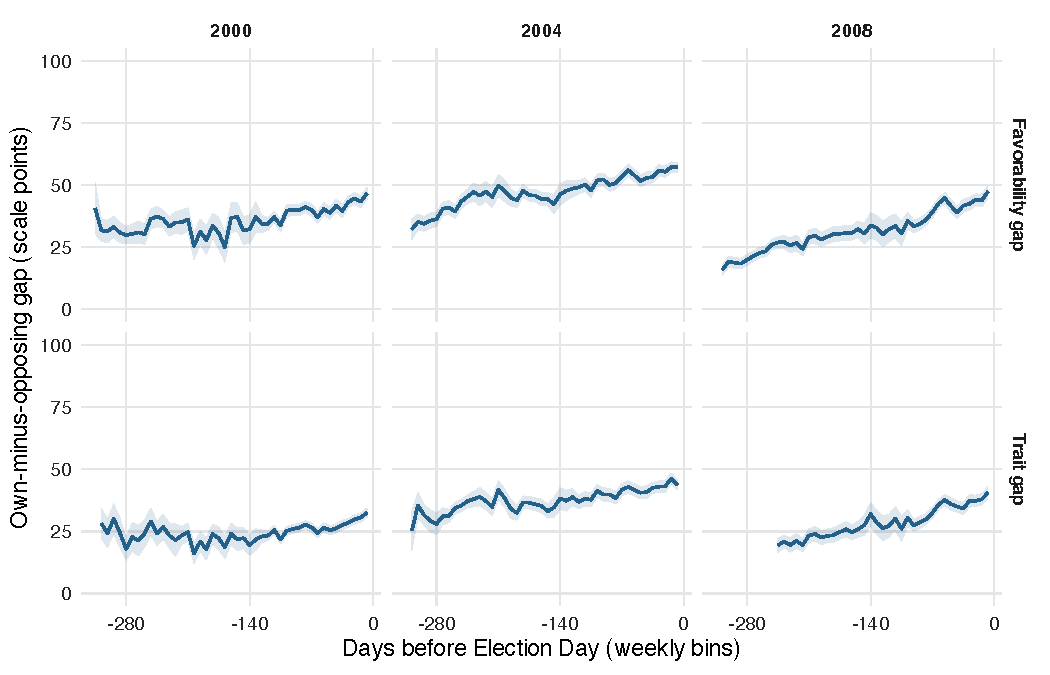
\includegraphics[width=\textwidth]{../figs/naes_gaps.pdf}
\caption{Candidate evaluation gaps during the election year. Weekly unweighted own-minus-opposing means among self-identified partisans; ribbons are respondent-level robust 95\% intervals. Each outcome requires paired candidate responses. Weeks with fewer than thirty usable observations are omitted. Trait batteries and response availability differ across elections.}
\label{fig:gaps}
\end{figure}

Candidate favorability gaps increase across the common autumn windows in all three NAES samples, but the size and precision differ. The increases are \FavZero{} points in 2000 (95\% CI \FavZeroCI{}), \FavFour{} in 2004 (\FavFourCI{}), and \FavEight{} in 2008 (\FavEightCI{}). The unadjusted 2008 interval includes zero. Standardization gives positive estimates in each year, conditional on the observed covariates and modeling choices (Table~\ref{tab:naes}). The numerical similarity between adjusted and unadjusted estimates does not establish that selection is absent.

\begin{table}[htbp]
\centering\small
\caption{Autumn changes in candidate evaluation gaps}
\label{tab:naes}
\begin{tabular}{llrrrr}
\toprule
Year & Measure & Early & Late & Change [95\% CI] & Adjusted change \\
\midrule
2000 & Favorability gap & 39.3 & 45.0 & 5.7 [2.7, 8.7] & 5.8 [3.0, 8.5] \\
2000 & Trait gap & 25.7 & 31.6 & 6.0 [4.2, 7.7] & 5.9 [4.4, 7.5] \\
2004 & Favorability gap & 54.2 & 57.1 & 3.0 [0.8, 5.2] & 3.2 [1.0, 5.4] \\
2004 & Trait gap & 41.6 & 44.9 & 3.3 [0.8, 5.8] & 3.8 [1.4, 6.3] \\
2008 & Favorability gap & 43.6 & 45.5 & 2.0 [-0.3, 4.2] & 2.4 [0.3, 4.4] \\
2008 & Trait gap & 36.6 & 39.3 & 2.7 [0.6, 4.7] & 2.9 [1.1, 4.6] \\
\bottomrule
\end{tabular}

\par\smallskip\begin{minipage}{\textwidth}\footnotesize
Early: September 1--14. Late: final fourteen days before Election Day. All quantities are scale points. Gaps are own minus opposing candidate; changes are late minus early. Primary estimates are unweighted. Adjusted contrasts standardize to complete-case autumn respondents. Both interval columns use state clustering. Samples and alternative inference are in the replication tables.
\end{minipage}
\end{table}

The weekly trajectories show why the window matters (Figure~\ref{fig:fav}). A change from early in the election year includes developments before the general-election period, including candidate selection and changing familiarity. It should not be read as the effect of a fixed dose of campaigning. Weekly observations also describe changing sets of respondents, not individual trajectories.

\begin{figure}[htbp]
\centering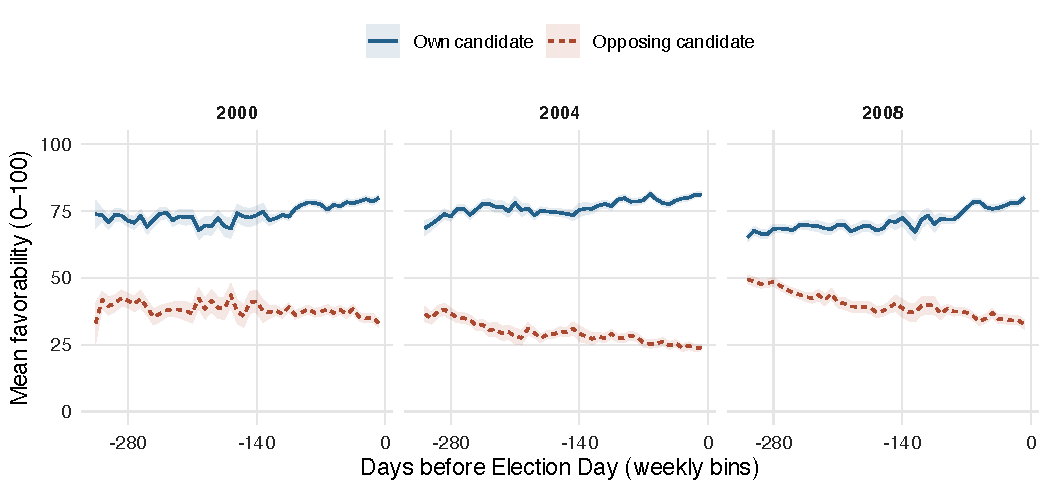
\includegraphics[width=\textwidth]{../figs/naes_fav.pdf}
\caption{Own- and opposing-candidate favorability during the election year. Weekly unweighted means among self-identified partisans with both ratings; ribbons are respondent-level robust 95\% intervals. Weeks with fewer than thirty paired observations are omitted.}
\label{fig:fav}
\end{figure}

Disaggregating the gap shows increases in own-candidate favorability and decreases in opposing-candidate favorability in each autumn comparison (Table~\ref{tab:decomp}). The opposing-candidate declines are numerically larger, but the interval for the sum of the two changes includes zero in each year. Thus these comparisons do not establish that declining evaluations of opponents consistently dominate improving evaluations of one's own candidate.

Trait gaps also increase (Table~\ref{tab:naes}; Figure~\ref{fig:traits}). Their components differ across elections. In 2004, the increase in own-candidate trait ratings is larger than the decline in opposing-candidate ratings. Complete-item and inherited-weight sensitivities widen the uncertainty around some trait comparisons, including intervals that cross zero (Appendix~\ref{app:sensitivity}). Question availability and the particular traits measured matter to the conclusion.

\begin{table}[htbp]
\centering\small
\caption{Own- and opposing-candidate components of autumn changes}
\label{tab:decomp}
\begin{tabular}{lllrr}
\toprule
Year & Measure & Candidate & Change [95\% CI] & $N$ \\
\midrule
2000 & Favorability & Own candidate & 2.6 [1.2, 4.1] & 4767 \\
2000 & Favorability & Opposing candidate & -3.0 [-5.2, -0.9] & 4767 \\
2000 & Traits & Own candidate & 1.0 [-0.1, 2.1] & 4889 \\
2000 & Traits & Opposing candidate & -5.0 [-6.1, -3.8] & 4889 \\
2004 & Favorability & Own candidate & 1.2 [0.2, 2.2] & 6159 \\
2004 & Favorability & Opposing candidate & -1.8 [-3.4, -0.3] & 6159 \\
2004 & Traits & Own candidate & 2.6 [1.3, 3.8] & 4031 \\
2004 & Traits & Opposing candidate & -0.7 [-2.2, 0.8] & 4031 \\
2008 & Favorability & Own candidate & 0.4 [-0.9, 1.8] & 4461 \\
2008 & Favorability & Opposing candidate & -1.5 [-2.9, -0.1] & 4461 \\
2008 & Traits & Own candidate & 0.5 [-0.7, 1.8] & 4450 \\
2008 & Traits & Opposing candidate & -2.1 [-3.4, -0.9] & 4450 \\
\bottomrule
\end{tabular}

\par\smallskip\footnotesize Unweighted late-minus-early changes, with state-clustered 95\% intervals. $N$ counts respondents in the two comparison periods. Both components use the same outcome-specific sample.
\end{table}

\begin{figure}[htbp]
\centering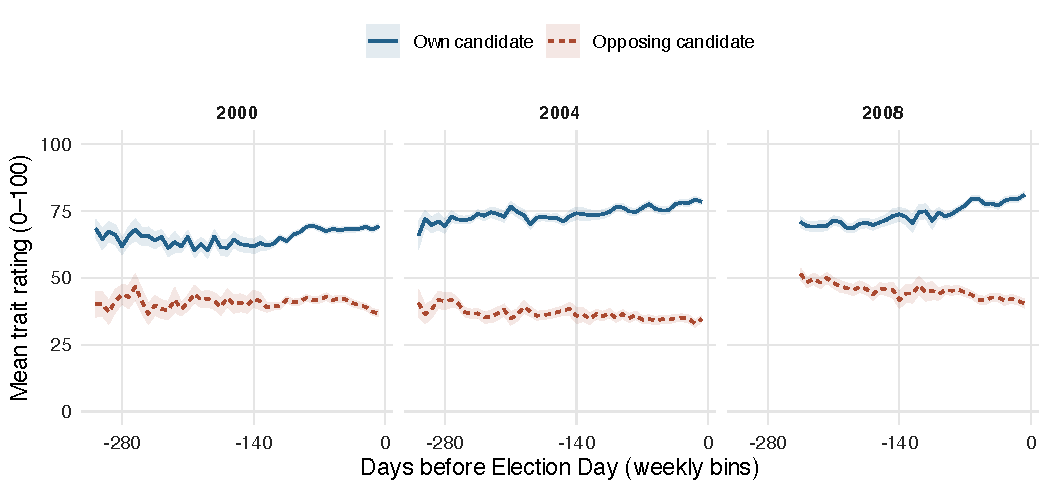
\includegraphics[width=\textwidth]{../figs/naes_trait.pdf}
\caption{Candidate trait evaluations. Each respondent's means use traits answered for both candidates. Batteries differ by year. Weekly unweighted means and respondent-level robust 95\% intervals; weeks with fewer than thirty usable observations are omitted.}
\label{fig:traits}
\end{figure}

The battleground comparisons show faster growth in trait gaps in each election, with pointwise intervals excluding zero (Table~\ref{tab:battleground}). Favorability gaps do not show the same consistency: only the 2008 slope difference has an interval excluding zero. These comparisons therefore provide mixed descriptive evidence for the expectation that candidate evaluations diverge more rapidly in competitive states. Differences in targeting, state electorates, and other campaign developments remain alternative explanations.

\begin{table}[htbp]\centering\small
\caption{Differences in trends between battleground and other states}\label{tab:battleground}
\begin{tabular}{llrr}
\toprule
Year & Measure & Slope difference [95\% CI] & $N$ \\
\midrule
2000 & Favorability gap & -0.5 [-1.5, 0.5] & 28164 \\
2000 & Trait gap & 1.4 [0.4, 2.4] & 25589 \\
2004 & Favorability gap & 1.1 [-0.2, 2.4] & 40678 \\
2004 & Trait gap & 1.1 [0.1, 2.2] & 26820 \\
2008 & Favorability gap & 1.3 [0.3, 2.2] & 34048 \\
2008 & Trait gap & 1.9 [0.7, 3.1] & 24359 \\
\bottomrule
\end{tabular}

\par\smallskip\begin{minipage}{\textwidth}\footnotesize
Battleground minus other-state linear slopes, in scale points per 100 days toward Election Day. Unweighted election-year pre-election observations; state-clustered 95\% intervals. Historical state lists are held fixed within each election. These are descriptive slope differences, not effects of campaign exposure.
\end{minipage}
\end{table}

Finally, perceived ideological positions and self--candidate distances provide descriptive context (Appendix~\ref{app:ideology}). They cannot adjudicate between learning, projection, and identity-based evaluation. Average positions can stay stable while some respondents learn and others change in the opposite direction. Item nonresponse and the coarse response scale further limit what a stable mean can reveal.

\section*{Discussion}
Our research connects to ongoing research showing that partisanship is a salient basis for group identity \citep{iyengar2012, freeze2012}. Across three presidential elections, the NAES data show growing candidate evaluation gaps during the common autumn periods, with differences in magnitude and precision. The weekly trajectories place those contrasts within the longer election year. The findings characterize a phenomenon worth explaining even when these data cannot identify its causes.

The components of the gap matter. Increasing warmth toward one's own candidate and declining evaluations of the opposing candidate both contribute, and their relative importance differs across elections and measures. A widening gap alone cannot establish that hostility is the dominant change. Nor do unfavorable evaluations of named candidates establish hostility toward ordinary supporters of the opposing party. Candidate evaluations can respond to perceived competence, policy disagreement, identity, and other considerations.

Partisan processing of information, strengthened attachments, and more salient identities remain plausible explanations for increasing candidate gaps. So do changing beliefs about candidates' competence and policy positions. Our perceived-position questions do not measure learning directly. Stable average placements could coexist with individual learning, offsetting changes, or changes too small for the response categories to capture. The data therefore leave learning's contribution open.

The comparisons across battleground and other states add geographic variation to the description. They do not isolate the effects of greater campaign activity. Similarly, a relationship between advertising volume and evaluations would require credible exposure measurement before it could be interpreted even as an association. A causal interpretation would further require an argument that separates advertising from campaign targeting and the other differences between places.

The broader 2008 candidate field shows why selection of eventual nominees matters. Opposing-party evaluations of Clinton rise over the observed year, while those of Obama and McCain decline (Appendix~\ref{app:field}). Several other candidates cease to be measured early. Their unobserved later ratings cannot be supplied by averaging the candidates who remain. The nominee trajectories therefore do not establish a common path for all presidential contenders.

The results concern observed respondents in three historical presidential campaigns. Changes in questionnaire availability, response patterns, and candidate familiarity affect which comparisons are informative. Covariate adjustment and alternative scoring choices probe particular sources of sensitivity, while leaving unmeasured differences unresolved. The descriptive contribution is to show the timing, components, and variation of candidate polarization clearly enough to guide more specific explanatory tests.

\clearpage
{\small
\setlength{\bibsep}{0pt}
\bibliographystyle{apsr}
\bibliography{polarcamp}
}
\clearpage
\appendix
\section{Sensitivity and response availability}\label{app:sensitivity}
Table~\ref{tab:sensitivity} varies weights, trait completeness, and the partisan sample. The inherited weights are researcher-created and are not treated as verified study weights. The full machine-readable tables additionally report individual traits, matched-sample unweighted comparisons, demographic composition, floor and ceiling frequencies, battleground trend differences, and alternative variance estimators. These are sensitivity analyses of descriptive contrasts; they do not create a counterfactual campaign exposure.

\begin{table}[htbp]\centering\small
\caption{Alternative NAES autumn specifications}\label{tab:sensitivity}
\begin{tabular}{lllrr}
\toprule
Year & Measure & Specification & Change [95\% CI] & $N$ \\
\midrule
2000 & Favorability gap & Inherited weight 1 & 5.9 [2.3, 9.5] & 4672 \\
2000 & Trait gap & Inherited weight 1 & 5.6 [3.7, 7.5] & 4788 \\
2000 & Favorability gap & Inherited weight 2 & 6.6 [2.2, 10.9] & 4672 \\
2000 & Trait gap & Inherited weight 2 & 5.9 [3.6, 8.2] & 4788 \\
2000 & Trait gap & All trait pairs & 5.9 [3.9, 8.0] & 4435 \\
2004 & Favorability gap & Inherited weight 1 & 2.9 [0.0, 5.8] & 6030 \\
2004 & Trait gap & Inherited weight 1 & 3.1 [-0.4, 6.7] & 3950 \\
2004 & Favorability gap & Inherited weight 2 & 2.6 [-0.2, 5.4] & 6030 \\
2004 & Trait gap & Inherited weight 2 & 2.8 [-0.5, 6.2] & 3950 \\
2004 & Trait gap & All trait pairs & 2.6 [-0.1, 5.2] & 3657 \\
2008 & Favorability gap & Inherited weight 1 & 1.1 [-1.7, 3.8] & 4258 \\
2008 & Trait gap & Inherited weight 1 & 2.5 [-0.1, 5.1] & 4247 \\
2008 & Favorability gap & Inherited weight 2 & 1.2 [-1.8, 4.2] & 4258 \\
2008 & Trait gap & Inherited weight 2 & 2.7 [-0.2, 5.6] & 4247 \\
2008 & Trait gap & All trait pairs & 2.8 [0.6, 5.0] & 4206 \\
2000 & Favorability gap & Including leaners & 4.9 [3.3, 6.6] & 7092 \\
2000 & Trait gap & Including leaners & 4.9 [3.8, 6.1] & 7289 \\
2004 & Favorability gap & Including leaners & 3.6 [1.8, 5.5] & 8450 \\
2004 & Trait gap & Including leaners & 4.0 [2.2, 5.9] & 5478 \\
2008 & Favorability gap & Including leaners & 1.8 [0.0, 3.6] & 6195 \\
2008 & Trait gap & Including leaners & 2.5 [0.8, 4.2] & 6174 \\
\bottomrule
\end{tabular}

\par\smallskip\footnotesize State-clustered 95\% intervals. Samples differ with weight and item availability. All trait pairs requires responses for every trait for both candidates. Including leaners uses the inherited seven-category identification measure.
\end{table}
\begin{figure}[htbp]\centering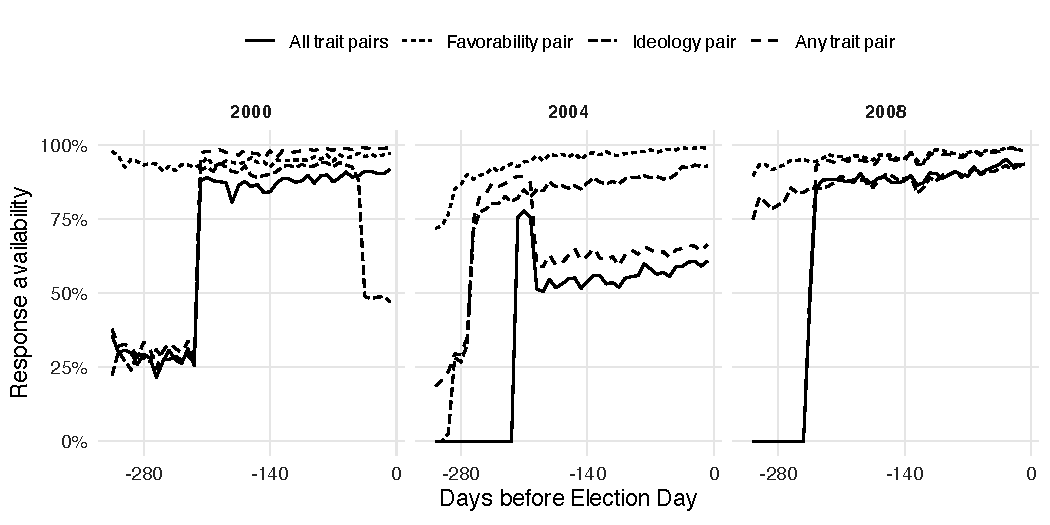
\includegraphics[width=.9\textwidth]{../figs/availability.pdf}
\caption{Weekly response availability among self-identified NAES partisans. The denominator includes respondents without usable outcome responses. Availability combines questionnaire fielding and respondent nonresponse.}
\end{figure}
\clearpage
\section{Perceived ideology}\label{app:ideology}
\begin{figure}[htbp]\centering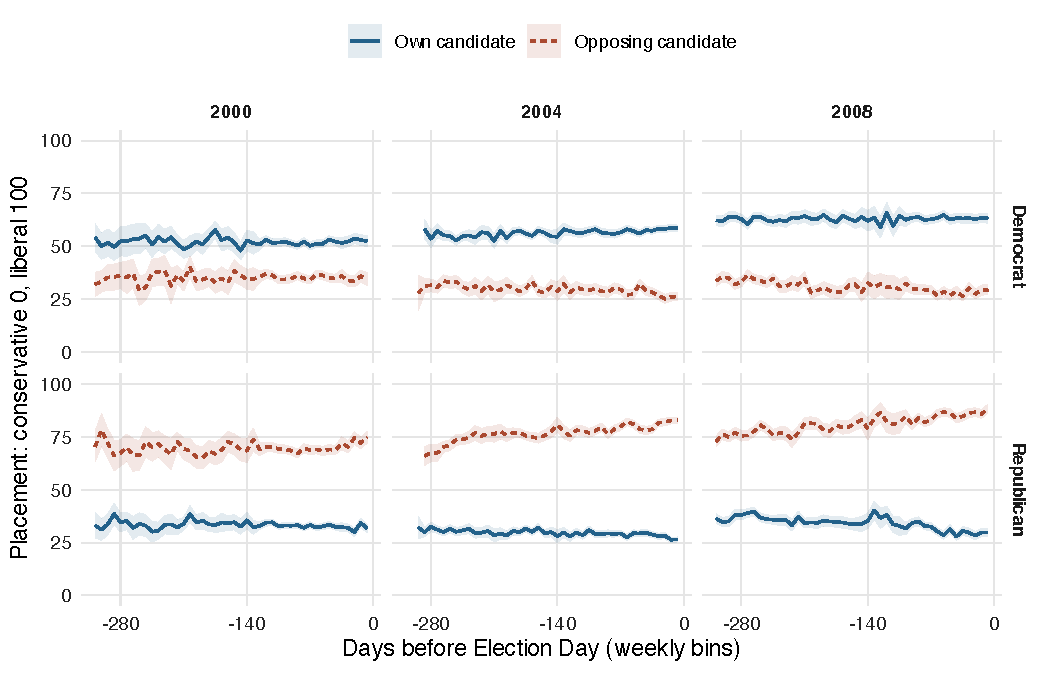
\includegraphics[width=\textwidth]{../figs/naes_ideology.pdf}
\caption{Perceived ideological placement of candidates. The scale runs from conservative (0) to liberal (100); rows separate Democratic and Republican respondents. Each series uses its available responses. Weekly unweighted means with respondent-level robust 95\% intervals, omitting weeks with fewer than thirty usable responses.}
\end{figure}
\begin{figure}[htbp]\centering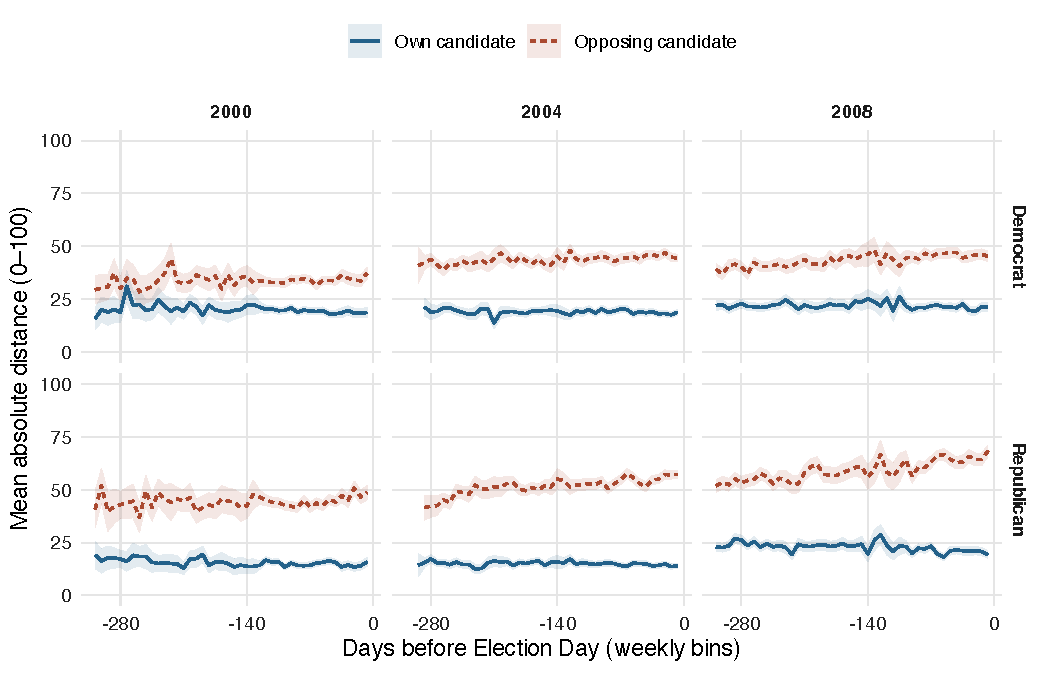
\includegraphics[width=\textwidth]{../figs/naes_distance.pdf}
\caption{Absolute distance between self-placement and perceived candidate placement. Each series requires both the respondent's and candidate's placement. A distance is not a measure of accuracy. Weekly unweighted means with respondent-level robust 95\% intervals, omitting weeks with fewer than thirty usable responses.}
\end{figure}

\clearpage
\section{The broader candidate field in 2008}\label{app:field}
The manuscript holds candidate identities fixed within each election. The figure below checks whether the 2008 nominee trajectories characterize other observed presidential contenders. Each candidate's available responses are retained separately. The nine candidates are those with verified presidential-contender favorability items in the archived workspace; this is not a census of all entrants. Biden and Palin ratings begin during the vice-presidential campaign and are excluded. Question availability does not define the active primary field: Clinton continues to be rated after her primary campaign, whereas Paul's item is asked only briefly in January. The official NAES08 phone codebook documents the fielding schedules.\footnote{\url{https://cdn.annenbergpublicpolicycenter.org/Downloads/NAES/PhoneSurvey/NAES08-Phone-Codebook.pdf}, variable directory, pp. 37--43.}

\begin{figure}[htbp]\centering
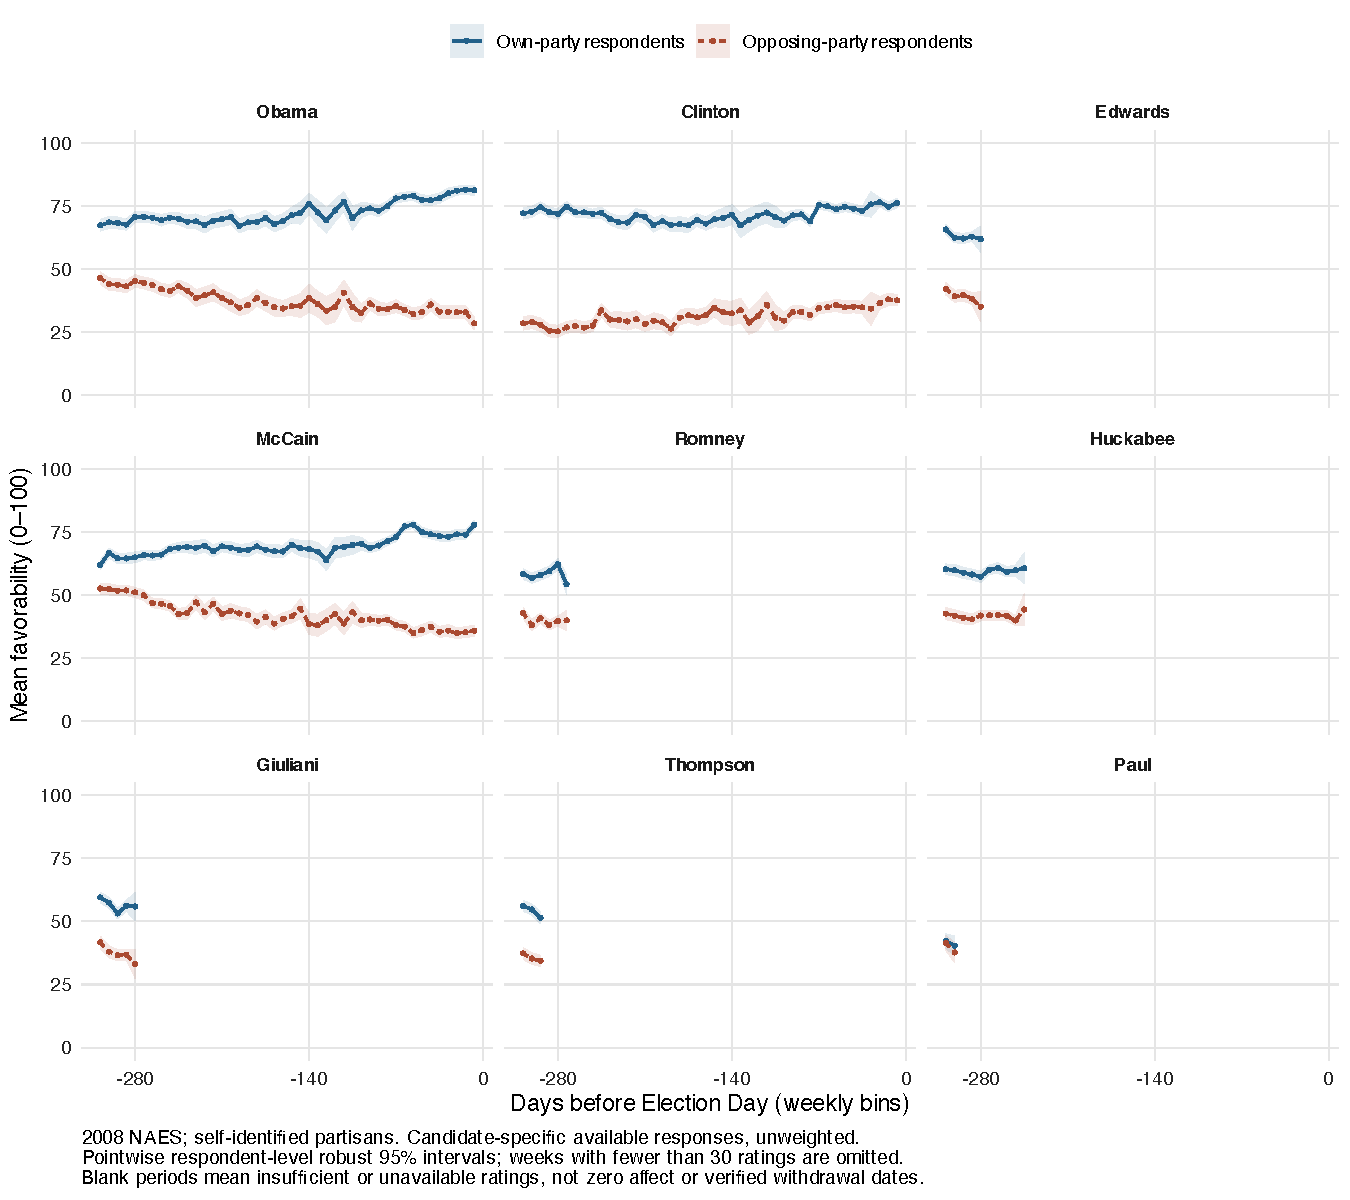
\includegraphics[width=\textwidth]{../figs/candidate_pool_2008.pdf}
\caption{Favorability of individual 2008 presidential contenders. Weekly unweighted means among self-identified partisans, separated by whether the respondent shares the candidate's party. Candidate-specific available responses; pointwise respondent-level robust 95\% intervals. Weeks with fewer than thirty ratings in a group are omitted. Blank periods are unobserved or insufficiently measured, not zero ratings or verified withdrawal dates.}
\end{figure}
\end{document}
